\documentclass{article}
\usepackage[utf8]{inputenc}

\title{EE2703 Assignment 4}
\author{Sakthi Harish D T}
\author{Author: Sakthi Harish D T, EE19B054}
\date{$10^{th}$ March,2021}

\usepackage{natbib}
\usepackage{graphicx}
\usepackage{listings}
\usepackage{amsmath}

\begin{document}

\maketitle{\hspace{3.5cm}\textbf{Fourier Approximations}}

\section{Abstract}
In this assignment, we will try to analyse 2 functions, $e^x$  and $cos(cos(x))$ over the interval $-2\pi$ to $4\pi$ using two methods, (i) By direct Integration , (ii) By Least Squares method.

\section{Introduction}
The Fourier Series of a function $f(x)$ with period $2\pi$ is computed as follows:
\begin{equation}
    f(x) = a_0 + \sum_{n=1}^{\infty}\{ a_ncos(nx) +b_nsin(nx)\}
\end{equation}
\newline
where , \newline


\[a_0 = \frac{1}{2\pi} \int_0^{2\pi}f(x)dx\]
\[a_n = \frac{1}{2\pi} \int_0^{2\pi}f(x)*\cos(nx)dx\]
\[b_n = \frac{1}{2\pi} \int_0^{2\pi}f(x)*\sin(nx)dx\]

Note that we treat exp(x) as a $2\pi$-periodic function while calculating the coefficients

\newpage
\section{Answers for questions in assignment}
\subsection{Creating the Python functions}
    We know that $cos(cos(x))$ is a periodic function with period $2\pi$ whereas $e^x$ is non-periodic. Therefore, the functions that will be generated from the Fourier series are $cos(cos(x))$ and $e^{x\%(2\pi)}$[Periodic extension of exp(x)] respectively.
    \lstset{language=Python}
    \lstset{label={lst:code_direct}}
    \lstset{basicstyle=\footnotesize}
    \begin{lstlisting}
        #function that returns exp(x)
        def exp_func(x):
            return(np.exp(x)) 
        #function that returns cos(cos(x))
        def cos_cos_func(x):
            return np.cos(np.cos(x))
    \end{lstlisting}
    Below are the plots of actual function along with the periodic extension of the same.
    Note that the cos(cos(x)) graphs coincides while the exp(x) does not. 
    \begin{figure}[h!]
    \centering
    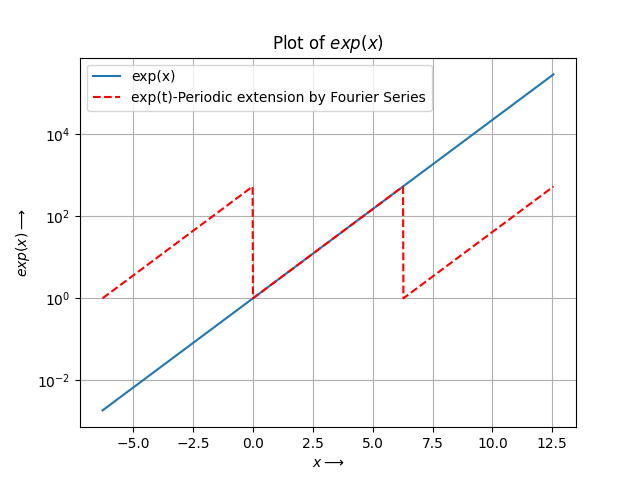
\includegraphics[scale=0.8]{exp(x).png}
    \label{fig:1(a)}
    \end{figure}
    \begin{figure}[h!]
    \centering
    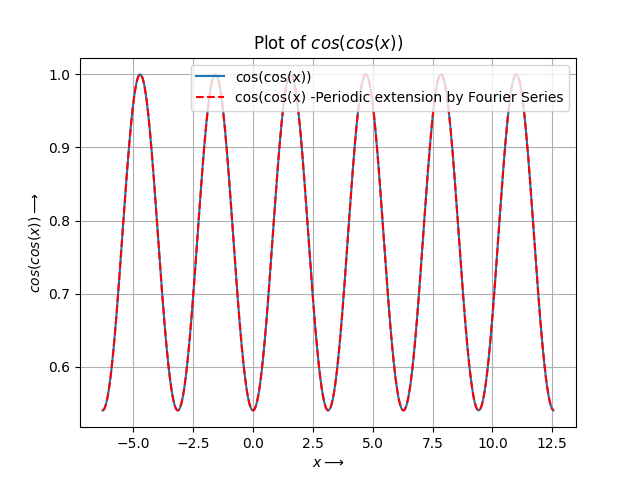
\includegraphics[scale=0.8]{coscosx.png}
    \label{fig:1(b)}
    \end{figure}
\newpage
\subsection{Generating Fourier Coefficients}
We generate the first 51 coefficients using the \textbf{scipy.integrate.quad} and the equations mentioned in the introduction section.They are saved in the following form as required by part 3:
\[
\begin{bmatrix}
    a_0 \\
    a_1 \\
    b_1 \\
    \dots \\
    a_{25} \\
    b_{25}
\end{bmatrix}
\]

\subsection{Analysing the Fourier Coefficients with plots}
The semilogy and log-log plots of the Coefficients obtained are plotted below. 
\newline
(a) We can see that $ \|b_n\|$ for cos(cos(x)) is almost 0. This is because cos(cos(x)) is an even function, whereas the integral involved in finding the $ b_n $ coefficient is odd in nature. $ b_n$ is not exactly 0 because of error in computational accuracy .\newline
(b) The coefficients for $e^x$ decay slower than that of $cos(cos(x))$ because rate of decay is directly proportional to the smoothness of the function. \newline
(c) The Log-log plot for Fourier coefficients of $e^x$ is nearly linear because the integrals,
\begin{equation}
\int_0^{2\pi} e^x cos(k x) dx = \frac{(e^{2\pi} - 1)}{(k^2 + 1)}    
\end{equation}
and 
\begin{equation}
\int_0^{2\pi} e^x sin(k x) dx = \frac{(-ke^{2\pi} + k)}{(k^2 + 1)}    
\end{equation}
have $1/n^2$ relation . The log-log plots of these functions are linear.

The semi-logy plot for Fourier Coefficients of $cos(cos(x))$ is linear as the integral converges to a Linear Combination of Bessel functions which are proportional to $e^x$.

\begin{figure}[h!]
    \centering
    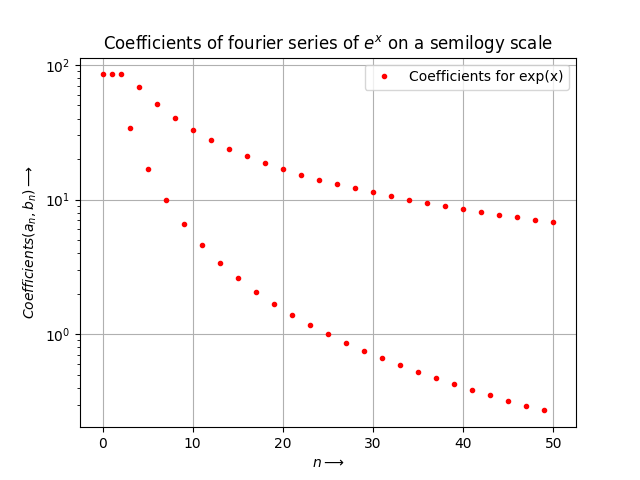
\includegraphics[scale=0.7]{expcoeff.png}
    \label{fig:1(b)}
\end{figure}
\begin{figure}[h!]
    \centering
    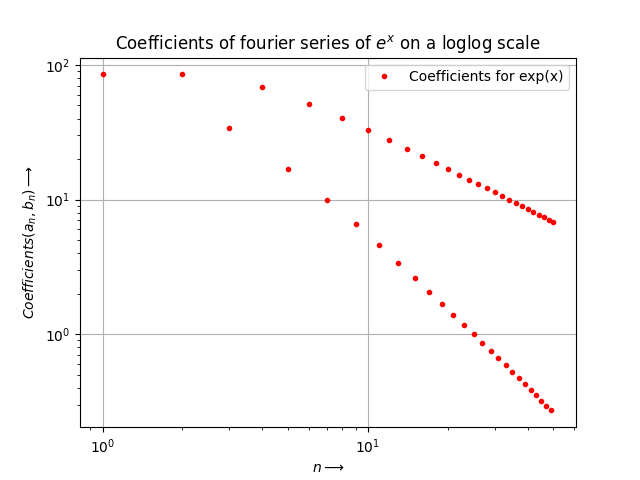
\includegraphics[scale=0.7]{expcoeff1.png}
    \label{fig:1(b)}
\end{figure}
\begin{figure}[h!]
    \centering
    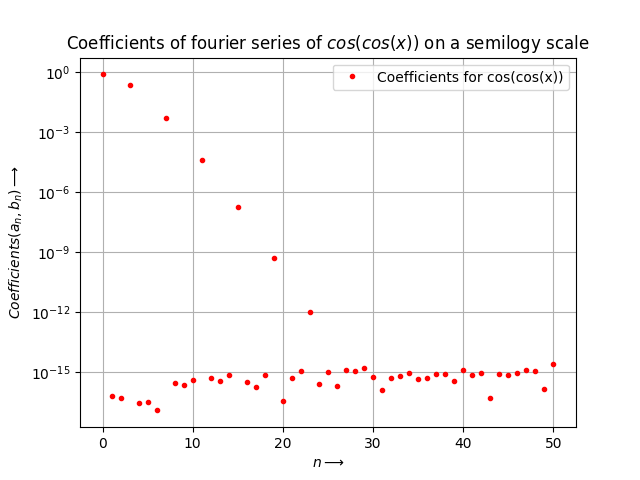
\includegraphics[scale=0.7]{coscoscoeff.png}
    \label{fig:1(b)}
\end{figure}
\begin{figure}[h!]
    \centering
    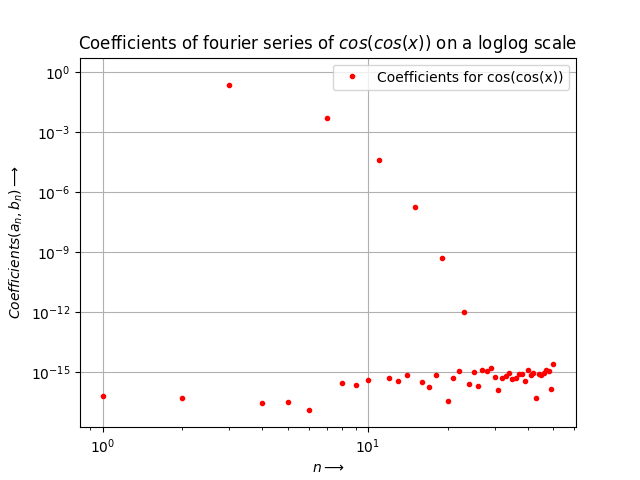
\includegraphics[scale=0.7]{coscoscoeff1.png}
    \label{fig:1(b)}
\end{figure}
\clearpage
\subsection{Least Squares Model}
Based on our previous week's work we now try the Least Squares Approach to this problem. We linearly choose 400 values of x in the range [0,2$\pi$).It should be noted that far better approximations were achieved when a larger value(~10000) was used instead of 400. 
We try to solve Equation (1) By using regression on these 400 values 
\[
\quad
\begin{pmatrix} 
1 & \cos(x_1) & \sin(x_1) & .... & \cos(25x_1) & \sin(25x_1)\\
1 & \cos(x_2) & \sin(x_2) & .... & \cos(25x_2) & \sin(25x_2)\\
... & ... & ... & .... & ... & ... \\
1 & \cos(x_{400}) & \sin(x_{400}) & .... & \cos(25x_{400}) & \sin(25x_{400})
\end{pmatrix}
\quad
\begin{pmatrix} 
a_0\\
a_1\\
b_1\\
...\\
a_{25}\\
b_{25}
\end{pmatrix}
=
\quad
\begin{pmatrix} 
f(x_1)\\
f(x_2)\\
...\\
f(x_{400})
\end{pmatrix}
\]

We call the matrix on the left side as \(A\) . We want to
solve \(Ac=b\) where \(c\) are the fourier coefficients.

\begin{lstlisting}

#This block estimates the Fourier series coefficients using the Least Square method

x=np.linspace(0,2*math.pi,401)
x=x[:-1] 
b1= exp_func(x)
b2= cos_cos_func(x)

#This block creates the matrix A
A=np.zeros((400,51))
A[:,0]=1
for k in range(1,26):
    A[:,2*k-1]=np.cos(k*x) 
    A[:,2*k]=np.sin(k*x)

c1= lstsq(A,b1)[0]
c2= lstsq(A,b2)[0]

\end{lstlisting}

\subsection{Analysing the resulting plots of the Least Squares model}
Below are the plots of the estimated coefficients using the Least squares model along with the actual coefficients for comparison.\newline 
\begin{figure}[h!]
    \centering
    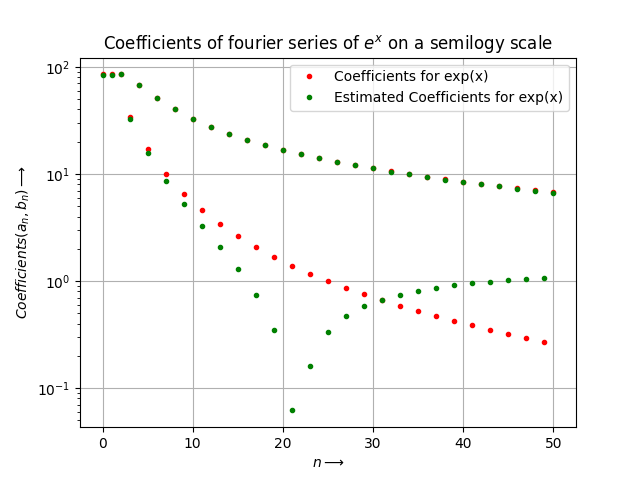
\includegraphics[scale=0.7]{estim_coeff1.png}
    \label{fig:1(b)}
\end{figure}
\begin{figure}[h!]
    \centering
    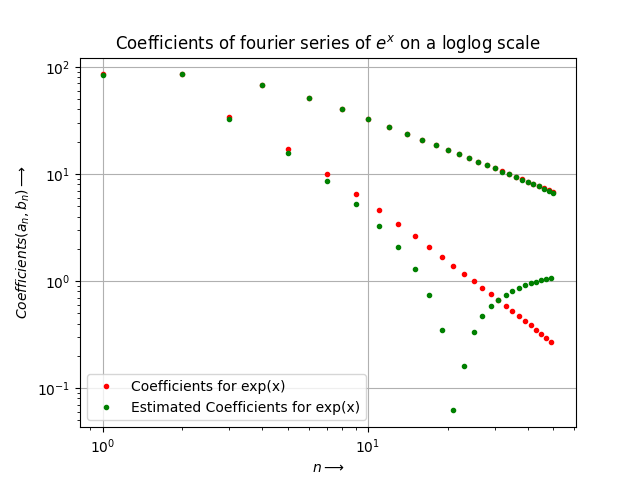
\includegraphics[scale=0.7]{estim_coeff2.png}
    \label{fig:1(b)}
\end{figure}
\begin{figure}[h!]
    \centering
    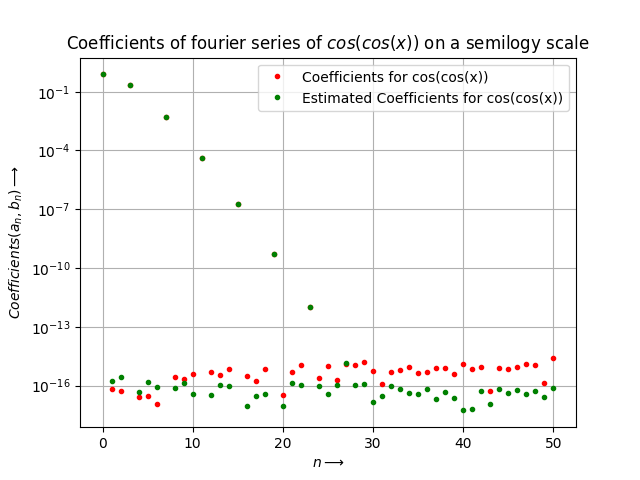
\includegraphics[scale=0.7]{estim_coeff3.png}
    \label{fig:1(b)}
\end{figure}
\begin{figure}[h!]
    \centering
    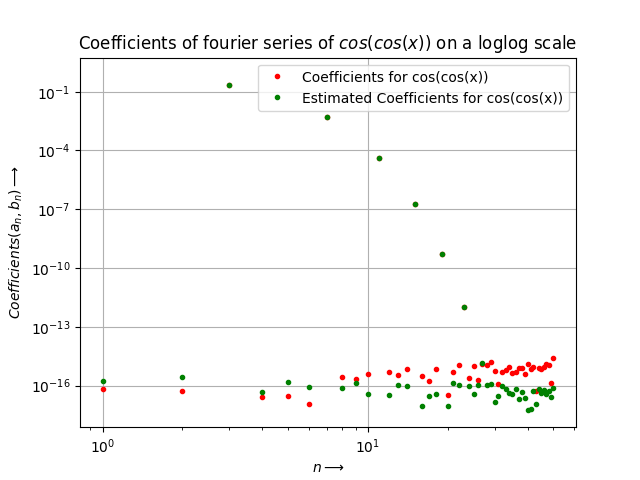
\includegraphics[scale=0.7]{estim_coeff4.png}
    \label{fig:1(b)}
\end{figure}
\clearpage
\subsection{Comparing Least squares with direct integration}
* The maximum absolute deviation for $e^x$ =1.3327308703353538\newline
* The maximum absolute deviation for cos(cos(x)) = 2.519109152022848e-15\newline
We can note that our Predictions for $e^x$ are very poor compared to that of cos(cos(x)). This can be fixed by sampling at a larger number of points.(say $10^5$ points)\newline 
But this would cost more computational load on the system.

\subsection{Regenerating the functions using the estimated coefficients}
Below are the plots for the functions generated using the estimated coefficients along with the actual functions for comparison.
\begin{figure}[h!]
    \centering
    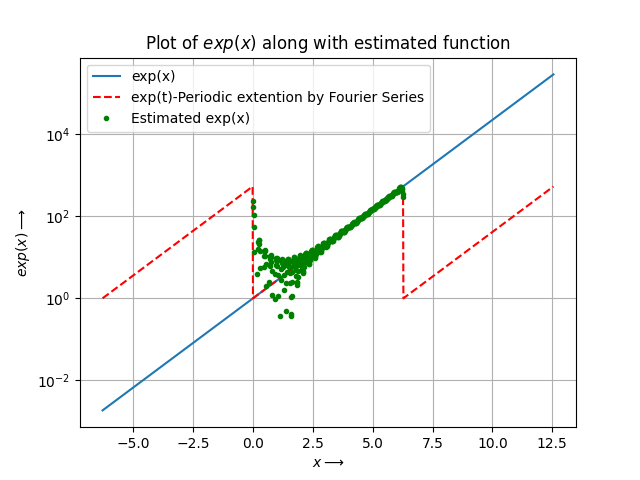
\includegraphics[scale=0.7]{exp_estim.png}
    \label{fig:1(b)}
\end{figure}
\begin{figure}[h!]
    \centering
    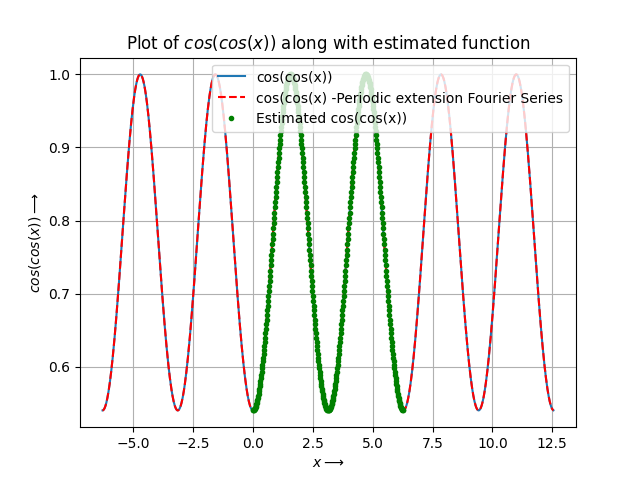
\includegraphics[scale=0.7]{coscos_estim.png}
    \label{fig:1(b)}
\end{figure}

It should be noted that $e^x$ is a non periodic function and Fourier series' exists only for periodic functions. Hence we have considered a variation of $e^x$ with period 2pi that has the actual value of $e^x$ only in the range [0,$2\pi$). Hence it is acceptable that there is a large discrepancy in the predicted value of $e^x$ at these boundaries
\newline
\newline
\section{Conclusion}
We have examined the case of approximating functions using their Fourier
coefficients upto a threshold. Whilst doing so, we perform the
same for two cases, one a continuous function, and the other a function
with finite discontinuities.
\newline
\newline
We adopted 2 methods in finding the respective Fourier coefficients,\newline
(i) direct evaluation of the Fourier series formula, \newline (ii) Least Square model .\newline \newline We notice close matching of the two methods in
case of \(\cos(\cos(x))\) while, there is a larger discrepancy in \(\exp(x)\).

\end{document}

